% Drawing 148/02-9 -- folder 148, batch 02, archive page 27 (PDF page 28).
% Transcription: planche de croquis à l'encre. En haut : un pentagone découpé en triangles depuis un sommet marqué, avec une flèche d'orientation ; une sphère entaillée de deux encoches, portant deux points ; une calotte triangulée dont les sommets sont numérotés $1$ à $6$ et $1'$ à $6'$. Au milieu : une anse (tube courbé) portant un trou et des chemins en tirets ; un tore à plusieurs contours repassés en gras ; un triangle sphérique de sommet $a$, avec $b_a$, $c_a$, $a'$. En bas : un tore, un anneau portant un point entouré, et une grande anse marquée $5$. Un long trait oblique traverse la planche.
% Kind: plate: triangulated pentagon, handles and tori with marked paths, numbered sphere, spherical triangle. Method 2 (schematic redraw from the facsimile). Status: partial.
% Notes: Schematic, from the grey render (upper two thirds) and a half-scale view (lower row): each figure at its place with its outline and its heavy strokes. Pentagon: five vertices, the top one a heavy dot, two diagonals from it, a doubled side at the right, a curled orientation arrow. Numbered cap: outline, heavy base stroke, the digits 1 to 6 inside and 1' to 6' around, placed as on the page (several are overinked: placed after the transcription). Spherical triangle: apex a, the two sides and the base, labels b_a, c_a, a' (the transcription also reads c_b; on the page the fourth label is not legible and is left out). The three words in the middle (« 4 sommets, 6 arêtes, 2 hexagones ») are text and left out. Still differs: the inner strokes of the handle, of the tori and of the cap (triangulation, dashed paths) are simplified, and the bottom row is drawn from a small view. Redrawn 2026-11-12 (issue 128): to check again.
% Coordinates: 1 unit = 1 mm = 1/100 of the crop width, y downwards as on the crop (bbox in page fractions: [0.09, 0.07, 0.91, 0.51]).
% Redrawn by Claude (claude-fable-5-2), issue #128, 2026-11-12; not checked by a human; not compiled (no TeX in the session).
% Rights: reproduces part of the work -- behind RENDER_TRANSCRIPTS, never published by itself.
\documentclass[tikz,border=3pt]{standalone}
\usepackage{amsmath,amssymb}
\usetikzlibrary{patterns,arrows.meta}
\tikzset{pencil/.style={black!45}, struck/.style={black!35}, mpt/.style={circle,draw,inner sep=1.3pt}, pt/.style={circle,fill,inner sep=0.9pt}, opt/.style={circle,draw,fill=white,inner sep=1.1pt}, Rd/.style={red!75!black}, Gn/.style={green!45!black}, Br/.style={brown!70!black}}
\begin{document}
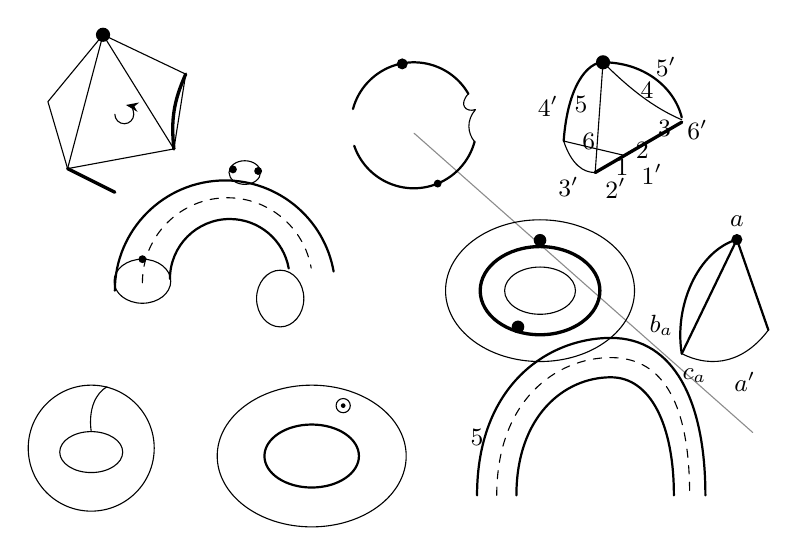
\begin{tikzpicture}[x=1mm,y=-1mm,line cap=round,line join=round,font=\small]
\draw[pencil] (55,16) -- (98,54);
% pentagon
\coordinate (p1) at (15.5,3.5);
\coordinate (p2) at (26,8.5);
\coordinate (p3) at (24.5,18);
\coordinate (p4) at (11,20.5);
\coordinate (p5) at (8.5,12);
\draw (p1) -- (p2) -- (p3) -- (p4) -- (p5) -- cycle;
\draw (p1) -- (p3);
\draw (p1) -- (p4);
\draw[very thick] (p2) to[bend right=15] (p3);
\draw[very thick] (p4) -- (17,23.5);
\fill (p1) circle [radius=0.9];
\draw[-{Stealth[length=1.6mm]}] (17,13.6) arc [start angle=180, end angle=-80, radius=1.2];
% handle
\draw[thick] (17,36) arc [start angle=180, end angle=350, radius=14];
\draw[thick] (24,34.5) arc [start angle=180, end angle=350, radius=7.6];
\draw[dashed] (20.5,35) arc [start angle=180, end angle=350, radius=10.8];
\draw (20.5,34.8) ellipse [x radius=3.6, y radius=2.8];
\draw (38,37) ellipse [x radius=3, y radius=3.6];
\draw (33.5,21) ellipse [x radius=2, y radius=1.5];
\fill (32,20.6) circle [radius=0.5];
\fill (35.2,20.8) circle [radius=0.5];
\fill (20.5,32) circle [radius=0.5];
% bitten sphere
\draw[thick] (61.9,11) arc [start angle=-30, end angle=-165, radius=8];
\draw[thick] (47.4,17.6) arc [start angle=161, end angle=15, radius=8];
\draw (61.9,11) .. controls (60.6,12.4) and (61.6,13.4) .. (62.8,13) .. controls (61.6,14.4) and (61.8,16) .. (62.7,17.1);
\fill (53.5,7.2) circle [radius=0.7];
\fill (58,22.4) circle [radius=0.5];
% numbered cap
\draw[thick] (74,17) .. controls (74.5,10) and (77,7) .. (79,7) .. controls (84,7) and (88,10) .. (89,14);
\draw[very thick] (78,21) -- (89,14.6);
\draw (74,17) .. controls (75,20) and (76.5,21) .. (78,21);
\draw (79,7) -- (78,21);
\draw (79,7) .. controls (83,11) and (86,13) .. (89,14.3);
\draw (74,17) -- (81.6,18.8);
\fill (79,7) circle [radius=0.9];
\node at (87,7.6) {$5'$};
\node at (72,12.6) {$4'$};
\node at (74.6,22.8) {$3'$};
\node at (80.6,23) {$2'$};
\node at (85.2,21.2) {$1'$};
\node at (91,15.6) {$6'$};
\node at (76.2,12.4) {$5$};
\node at (84.6,10.6) {$4$};
\node at (77.2,17) {$6$};
\node at (86.8,15.4) {$3$};
\node at (84,18.2) {$2$};
\node at (81.4,20.4) {$1$};
% torus
\draw (71,36) ellipse [x radius=12, y radius=9];
\draw[very thick] (71,36) ellipse [x radius=7.6, y radius=5.6];
\draw (71,36) ellipse [x radius=4.5, y radius=3];
\fill (71,29.6) circle [radius=0.8];
\fill (68.2,40.6) circle [radius=0.8];
% spherical triangle
\coordinate (a) at (96,29.5);
\coordinate (b) at (89,44);
\coordinate (c) at (100,41);
\draw[thick] (a) .. controls (91,31) and (88,38) .. (b);
\draw[thick] (a) -- (b);
\draw[thick] (a) -- (c);
\draw (b) .. controls (93,46) and (97,45) .. (c);
\fill (a) circle [radius=0.7];
\node at (96,27.2) {$a$};
\node at (86.4,40.4) {$b_a$};
\node at (90.6,46.8) {$c_a$};
\node at (97,47.6) {$a'$};
% bottom row
\draw (14,56) circle [radius=8];
\draw (14,56.5) ellipse [x radius=4, y radius=2.6];
\draw (14,53.9) .. controls (13.6,51) and (14.6,49) .. (16,48.2);
\draw (42,57) ellipse [x radius=12, y radius=9];
\draw[thick] (42,57) ellipse [x radius=6, y radius=4];
\draw (46,50.6) circle [radius=0.9];
\fill (46,50.6) circle [radius=0.3];
\draw[thick] (63,62) .. controls (63,48) and (72,42) .. (80,42) .. controls (88,42) and (92,50) .. (92,62);
\draw[thick] (68,62) .. controls (68,52) and (74,47) .. (80,47) .. controls (85,47) and (88,53) .. (88,62);
\draw[dashed] (65.5,62) .. controls (65.5,50) and (73,44.5) .. (80,44.5) .. controls (87,44.5) and (90,51) .. (90,62);
\node at (63,54.6) {$5$};
\end{tikzpicture}
\end{document}
